\documentclass[12pt,letterpaper]{article}

\usepackage[utf8]{inputenc}
\usepackage[spanish]{babel}
\usepackage{times}
\usepackage[left=3cm,top=2.5cm,bottom=2.5cm,right=2.5cm]{geometry}
\usepackage{graphicx}
\title{EV\_ 2\_ 4\_ giro\_ de\_ un\_ motor\_ de\_ corriente\_ directa.}


\begin{document}
\maketitle




\paragraph{ UNIVERSIDAD POLITÉCNICA DE LA ZONA METROPOLITANA DE GUADALAJARA}

\
\begin{figure}[h!]
\begin{center}


\includegraphics[scale=0.8]{Upzmg.png} 
\label{Upzmg}


\end{center}
\end{figure}


\

\large{Perez de Alba Santiago Eduardo.\\
\

Curso: Sep-Nov 2019.

\
Carrera: Ingeniería en Mecatronica.\

Docente: Moran Garabito Carlos Enrique}

\newpage

\section{Marco teórico:}
\

Los motores eléctricos de corriente continua son mas versátiles debido a su fácil control de posición, par y velocidad para aplicaciones de control y automatización de procesos. Es esencialmente una máquina que convierte energía eléctrica en movimiento o trabajo mecánico, a través de electromagnéticos.
\

\begin{figure}[h!]
\begin{center}
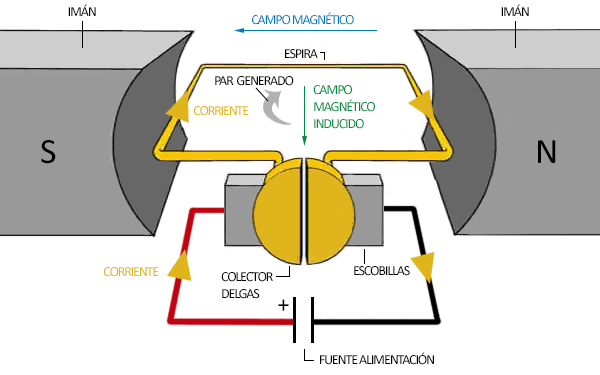
\includegraphics[scale=0.5]{images.png} 
\caption{Funcionamiento por electromagnetismo.}
\end{center}
\end{figure}


\

Para funcionar un motor se vale de las fuerzas de atracción y repulsión que existen entre los polos. Entonces, todo motor que esta formado con polos alternados entre el estator y el rotor, ya que los polos magnéticos iguales se repelen, y polos magnéticos diferentes se atraen, produciendo así el movimiento de rotación.
\

Un motor funciona en base a dos principios: El de inducción, que señala, que si un conductor se mueve a través de un campo magnético o esta situado en las proximidades de otro conductor por el que no circula una corriente de intensidad variable, se induce una corriente eléctrica en el primer conductor. Y el principio de Ampere que establece: que si una corriente pasa a través de un conductor situado en el interior de un campo magnético, éste ejerce una fuerza mecánica o f.e.m. (fuerza electromotriz), sobre el conductor.
\

\newpage

El movimiento giratorio de los motores C.D se basa en el empuje derivado de la repulsión y atracción entre polos magnéticos.
\ 

\begin{figure}[h!]
\begin{center}
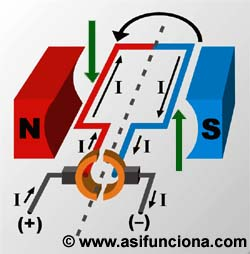
\includegraphics[scale=0.6]{Motor.jpg} 
\caption{Funcionamiento de motor.} 
\end{center}
\end{figure}


\end{document}